\documentclass[lang=cn,newtx,10pt,scheme=chinese]{elegantbook}

\title{模板 elegantbook.cls 使用示例}
\subtitle{为使用 \LaTeX{} 制作课程复习材料而生}

\author{kissdata}

% \date{2023/1/11}
% \version{1.0}

\extrainfo{感谢模板作者:Ethan Deng}

\setcounter{tocdepth}{3}

\logo{logo-blue.png}
\cover{cover.jpg}

\usepackage{array}
\newcommand{\ccr}[1]{\makecell{{\color{#1}\rule{1cm}{1cm}}}}

% 修改标题页的橙色带
\definecolor{customcolor}{RGB}{32,178,170}
\colorlet{coverlinecolor}{customcolor}
\usepackage{cprotect}

\addbibresource[location=local]{reference.bib} % 参考文献

\begin{document}
	
	\maketitle % 封面

这是一个教学使用 tex 开源模块库 elegantbook 的案例。为什么用这玩意儿?\\
因为它在 2022 年底 “定型” 了,最终版本 v4.5。你可以在
\href{https://github.com/ElegantLaTeX/ElegantBook/releases}{github.com/ElegantLaTeX/ElegantBook} 下载。

	\frontmatter  % 目录链接
	\tableofcontents % 目录
	\mainmatter % 章节带序号,目录带页码



\chapter{文章整体布局框架}
	
	\section{去除无效努力}
	
	你的知识是课本的,整理的本质只是做个复读机,不要花精力维护封面、来源、出处这些。也不方便打印下来看。
	在目录前加一页代替封面,随便写点介绍更好。方法是,把文字内容写在 \lstinline|\frontmatter| 前面。
	具体参考 test1.tex。

	\section*{备注}
	
	加载图片方法。

\begin{lstlisting}[language=tex]
\begin{figure}[!htb]
	\centering
	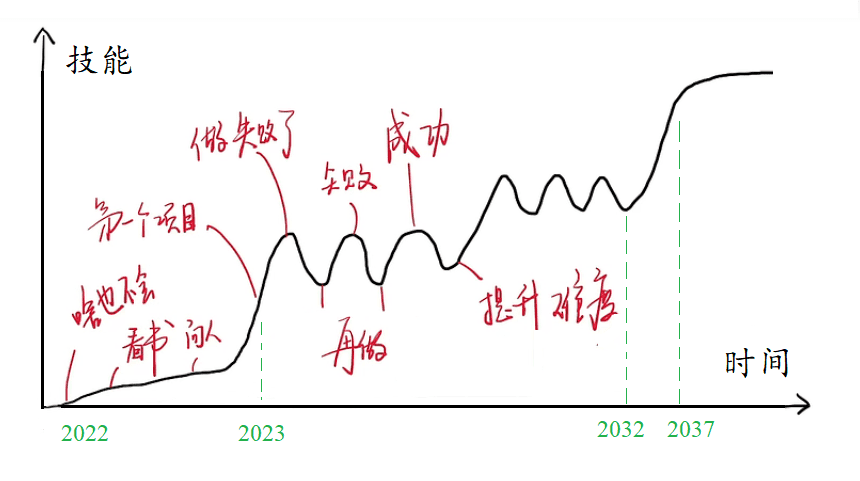
\includegraphics[width=0.9\textwidth]{life.png}
\end{figure}
\end{lstlisting}

图片在 image 目录,没有对应名字的图会报错。效果

	\begin{figure}[!htb]
		\centering
		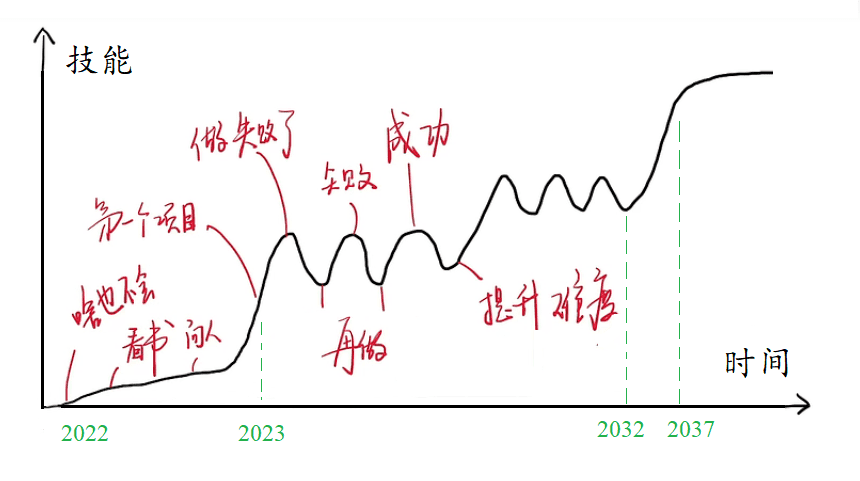
\includegraphics[width=0.9\textwidth]{life.png}
	\end{figure}


\chapter{还没想到}

已经够用了,以后用到再说



\nocite{*}
\printbibliography[heading=bibintoc, title=\ebibname]

\appendix 

\chapter{没什么想说的}

	
\end{document}